\chapter{Analisi dei risultati}\label{chap:results}


\noindent Questo capitolo presenta e interpreta i risultati. L'ordine non è per metrica ma per
\emph{caso}: la potatura che non perde nulla, il confronto con il criterio di ridondanza della
teoria classica, la potatura che produce il guadagno e il confine oltre il quale il guadagno non
si realizza, e il meccanismo che rende conto dei casi osservati. Da quel meccanismo discende un
criterio diagnostico, di cui il capitolo tenta la verifica su una famiglia indipendente; seguono i
risultati negativi e l'analisi del costo, che mostra perché la riduzione delle regole non basti a
garantire un risparmio di tempo. La lettura d'insieme, gli esiti delle ipotesi e i limiti
dell'evidenza sono oggetto del capitolo di discussione.

% =======================================================================================
\section{La strategia che non perde nulla}\label{sec:res-vetocover}

La condizione \Vtwo{} è l'unico criterio di potatura che offra una garanzia. La sua applicazione
è stata verificata su \num{113} configurazioni --- \num{111} distribuite su tre famiglie e
\num{2} su una quarta famiglia indipendente (\autoref{sec:physician}) --- con la condizione
che l'output del sistema sia \emph{identico} a quello della configurazione di partenza --- non
soltanto equivalente nelle metriche aggregate, ma identico cella per cella.

\begin{table}[htbp]
\centering
\caption{Applicazione della condizione \Vtwo{} su tre famiglie. ``Identiche'' è il numero di
configurazioni in cui corrette, errori e copertura coincidono esattamente con la configurazione
di partenza.}
\label{tab:res-vetocover}
\footnotesize
\begin{tabular}{llrrrrr}
\toprule
famiglia & soglia & $n$ & $N$ & riduzione & $\Delta$ corrette & identiche \\
\midrule
Bridges    & 3  & 10 & \num{1830}  & \SI{11.7}{\percent} & 0 & \textbf{10/10} \\
Bridges    & 9  & 10 & \num{8961}  & \SI{17.1}{\percent} & 0 & \textbf{10/10} \\
Bridges    & 15 & 10 & \num{18844} & \SI{20.8}{\percent} & 0 & \textbf{10/10} \\
Glass      & 3  & 25 & \num{1511}  & \SI{2.6}{\percent}  & 0 & \textbf{25/25} \\
Glass      & 9  & 25 & \num{11648} & \SI{7.4}{\percent}  & 0 & \textbf{25/25} \\
Glass      & 15 & 25 & \num{27445} & \SI{8.6}{\percent}  & 0 & \textbf{25/25} \\
Restaurant & 3  &  8 & 25          & \SI{0.0}{\percent}  & 0 & \textbf{8/8} \\
Restaurant & 6  &  8 & 124         & \SI{1.6}{\percent}  & 0 & \textbf{8/8} \\
\midrule
\textbf{totale} & & \textbf{113} & & & \textbf{0} & \textbf{113/113} \\
\bottomrule
\end{tabular}
\end{table}

Il risultato va letto nei due sensi. Nel senso positivo, è la conferma che la condizione \Vtwo{}
è corretta: una potatura \emph{esatta} è possibile, e la sua applicazione non altera di una sola
cella il comportamento del sistema. Nel senso negativo, la \autoref{tab:res-vetocover} mostra
anche il prezzo: la riduzione è nulla su Restaurant a soglia 3, inferiore al \SI{3}{\percent} su
Glass a soglia 3, e non supera il \SI{20.8}{\percent} in alcun caso.

La verifica è stata condotta anche in forma indipendente, controllando su stati reali del dataset
--- e non soltanto per implicazione logica --- che per ogni regola rimossa esistesse una regola
coprente sopravvissuta in grado di esercitare il veto sugli stessi testimoni. La verifica ha
coperto \num{1242321} terne, con zero discrepanze.

% =======================================================================================
% =======================================================================================
\section{La riduzione classica, e perché non è sicura}\label{sec:res-classical}

Il termine di paragone più ovvio per una potatura è la riduzione di ridondanza della teoria
classica delle dipendenze funzionali: una regola $X \to A$ è superflua se un'altra regola
$Y \to A$ ha $Y$ sottoinsieme proprio di $X$, perché $X \to A$ si ottiene per augmentazione
(\autoref{sec:rule-reduction}). Il criterio è sintattico e ignora le soglie; è stato implementato
come strategia (\str{classical-cover}) e misurato sulle medesime configurazioni di Bridges a
soglia 9, con la medesima ricetta di accoppiamento delle altre campagne.

\begin{table}[htbp]
\centering
\caption{Riduzione classica (\str{classical-cover}) su Bridges a soglia 9, prima ripetizione:
l'insieme passa da \num{8961} a \num{230} regole in tutte e cinque le configurazioni
(\SI{97.4}{\percent}). Ogni riga confronta la configurazione di partenza con quella potata.}
\label{tab:res-classical}
\footnotesize
\begin{tabular}{@{}lrrrrr@{}}
\toprule
configurazione & copertura & accuratezza & corrette & errori & tempo (\si{\second}) \\
\midrule
\texttt{bridges\_14\_1} & $0.714 \to 0.571$ & $0.643 \to 0.500$ & $9 \to 7$   & $1 \to 3$   & $9.9 \to 0.3$ \\
\texttt{bridges\_28\_1} & $0.714 \to 0.643$ & $0.643 \to 0.429$ & $18 \to 12$ & $2 \to 6$   & $32.0 \to 0.6$ \\
\texttt{bridges\_42\_1} & $0.595 \to 0.595$ & $0.524 \to 0.429$ & $22 \to 18$ & $3 \to 7$   & $36.9 \to 0.7$ \\
\texttt{bridges\_56\_1} & $0.679 \to 0.571$ & $0.589 \to 0.321$ & $33 \to 18$ & $4 \to 10$  & $56.9 \to 1.0$ \\
\texttt{bridges\_70\_1} & $0.529 \to 0.500$ & $0.457 \to 0.357$ & $32 \to 25$ & $6 \to 12$  & $54.9 \to 1.0$ \\
\midrule
totale & & & \textbf{114} $\to$ \textbf{80} & \textbf{16} $\to$ \textbf{38} & \\
\bottomrule
\end{tabular}
\end{table}

Il risultato va nella direzione opposta a quella che il solo numero di regole rimosse
suggerirebbe. La riduzione è del \SI{97.4}{\percent} --- da \num{8961} a \num{230} regole, molto
oltre il \SI{20.9}{\percent} della classe garantita e oltre l'\SI{84}{\percent} della strategia
aggressiva --- e il tempo di esecuzione cala di oltre cinquanta volte; ma l'output cambia in
\emph{tutte} le configurazioni, la copertura scende, l'accuratezza mediana perde \num{14.3} punti,
le imputazioni corrette passano da \num{114} a \num{80} e gli errori da \num{16} a \num{38}. La
circostanza va letta con la numerosità che ha: con cinque configurazioni il test esatto dà
$p = \num{0.0625}$, e nessuna delle cinque migliora, ma la soglia convenzionale di significatività
non è raggiunta. Ciò che il confronto stabilisce non è una differenza statisticamente significativa
rispetto al criterio classico, ma che il criterio classico \emph{non è innocuo}: la sua applicazione
altera il comportamento del sistema in ogni caso osservato.

La spiegazione è quella argomentata nella \autoref{sec:rule-reduction}. Il criterio classico
rimuove regole che il sistema usava, perché la relazione di sussunzione che lo fonda non tiene
conto né della \emph{direzione} delle soglie sul lato destro né dell'\emph{ampiezza} di quelle sul
lato sinistro: la regola dichiarata superflua può generare candidati, e la regola che la sussume
può essere più severa e quindi non implicarne il veto. La condizione \Vtwo{} è l'analogo operativo
di quella relazione, ma richiede soglie più larghe a sinistra e non più larghe a destra, cioè la
direzione opposta.

La conseguenza per la lettura del lavoro è duplice. Sul piano teorico, il confronto è la verifica
empirica della distinzione fra ridondanza dichiarativa e sicurezza operativa. Sul piano della
valutazione, mostra perché la riduzione non possa essere l'unico indicatore di una strategia: un
criterio che rimuove il \SI{97}{\percent} delle regole peggiorando il risultato è, per gli
obiettivi di questo lavoro, peggiore di uno che ne rimuove il \SI{17}{\percent} senza toccarlo.

\section{La strategia che produce il guadagno}\label{sec:res-a5b}

La combinazione \str{A5b}, che abbina un riordino delle regole a soglia di destra nulla a una
potatura adattiva, è stata valutata sull'intera griglia di Bridges: cinque livelli di
incompletezza, cinque esecuzioni indipendenti, due soglie.

\begin{table}[htbp]
\centering
\caption{\str{A5b} su Bridges, griglia completa. Confronto appaiato con la medesima
configurazione non potata.}
\label{tab:res-a5b}
\footnotesize
\begin{tabular}{lrrrrrr}
\toprule
soglia & $n$ & riduzione RFD & $\Delta$ corrette & $\Delta$ errori & $\Delta$ precisione & accelerazione \\
\midrule
9  & 25 & \SI{81.2}{\percent} & $+32$ & $-40$ & $+0.050$ & \num{9.0}$\times$ \\
15 & 25 & \SI{87.2}{\percent} & $+37$ & $-32$ & $+0.038$ & \num{17.5}$\times$ \\
\midrule
\textbf{totale} & \textbf{50} & \textbf{\SI{84.2}{\percent}} & $\mathbf{+69}$ & $\mathbf{-72}$ & $+0.044$ & \num{11.0}$\times$ \\
\bottomrule
\end{tabular}
\end{table}

Il test di Wilcoxon signed-rank sulle corrette dà, sull'insieme delle \num{50} configurazioni,
$n = 39$, $W^+ = 589$, $W^- = 191$, $p = \num{0.0053}$; sugli errori, $p = 2.5\cdot 10^{-6}$. Separando
per soglia il quadro è più sfumato e va riportato: a soglia 9 il test dà $p = \num{0.0562}$
($n = 18$) e a soglia 15 $p = \num{0.0484}$ ($n = 21$), sicché \emph{nessuna delle due soglie da
sola} è conclusiva al livello del \SI{5}{\percent}, mentre l'insieme delle configurazioni lo è
con ampio margine. La ragione è che in una parte delle configurazioni la potatura è neutra, e il
test vede soltanto le differenze non nulle.

Il risultato va confrontato con quello della \autoref{sec:res-vetocover}. La strategia garantita
non altera nulla e riduce poco; \str{A5b} riduce molto e \emph{migliora} il risultato. Le due
strategie non sono alternative sullo stesso asse: rispondono a due domande diverse.

% =======================================================================================
\section{Il confine: dove il guadagno non si realizza}\label{sec:res-boundary}

La medesima strategia, applicata a Glass e Restaurant con la stessa taratura, produce un
danneggiamento sistematico.

\begin{table}[htbp]
\centering
\caption{Effetto della potatura aggressiva su tutte le famiglie. La taratura è la medesima
($\alpha = 0.85$).}
\label{tab:res-boundary}
\footnotesize
\begin{tabular}{llrrrr}
\toprule
famiglia & $n$ & riduzione RFD & $\Delta$ corrette & $\Delta$ copertura & esito \\
\midrule
Bridges    & 50 & \SI{84.2}{\percent} & $\mathbf{+69}$ & $-0.003$ & \textbf{migliora} \\
Glass      & 45 & \SI{82.8}{\percent} & $-54$          & $-0.034$ & danneggia \\
Restaurant & 18 & \SI{44.2}{\percent} & $-12$          & $-0.005$ & danneggia \\
\bottomrule
\end{tabular}
\end{table}

La causa è precisata dal segno della variazione di copertura: su Glass la potatura riduce le
imputazioni effettuate di circa un terzo, e il danno è quindi una \emph{perdita di copertura},
non un peggioramento della qualità di ciò che viene imputato. Su Bridges, invece, la copertura
non cala.

Una taratura più conservativa della medesima strategia --- ottenuta alzando la soglia di
stabilità del parametro di potatura --- elimina il danneggiamento su Glass e Restaurant, al
prezzo di una riduzione molto inferiore:

\begin{table}[htbp]
\centering
\caption{La medesima strategia con taratura conservativa ($\alpha = 0.99$) su Glass e Restaurant,
griglia completa. ``Identiche'' indica le configurazioni in cui corrette, errori e copertura
coincidono con la configurazione di partenza.}
\label{tab:res-gentle}
\footnotesize
\begin{tabular}{lrrrrr}
\toprule
famiglia & config. & identiche & $\Delta$ corr. & $\Delta$ err. & riduz.\ (mediana / massima) \\
\midrule
Glass      & 75 & \textbf{74/75} & 0   & $-1$ & \SI{0.1}{\percent} / \SI{52.9}{\percent} \\
Restaurant & 22 & \textbf{20/22} & $-1$ & $-2$ & \SI{0.0}{\percent} / \SI{45.2}{\percent} \\
\midrule
\textbf{totale} & \textbf{97} & \textbf{94/97} & $\mathbf{-1}$ & $\mathbf{-3}$ & \SI{0.0}{\percent} / \SI{52.9}{\percent} \\
\bottomrule
\end{tabular}
\end{table}

Il confronto fra la \autoref{tab:res-boundary} e la \autoref{tab:res-gentle} è istruttivo: la
stessa strategia passa da $-54$ a $-1$ imputazioni corrette su Glass al variare di un solo
parametro. La spiegazione di questa sensibilità è l'oggetto della sezione successiva.

Un elemento della \autoref{tab:res-gentle} va sottolineato perché limita la portata del
risultato: la riduzione \emph{mediana} è nulla. Su più della metà delle configurazioni la
strategia conservativa non rimuove alcuna regola. Il beneficio si concentra in \num{27}
configurazioni su \num{97}, dove è sostanzioso. Ciò che la taratura conservativa garantisce su
tutte le configurazioni non è la riduzione, ma l'assenza di perdite rilevanti.

% =======================================================================================
\section{Il meccanismo}\label{sec:mechanism}

\begin{figure}[htbp]
\centering
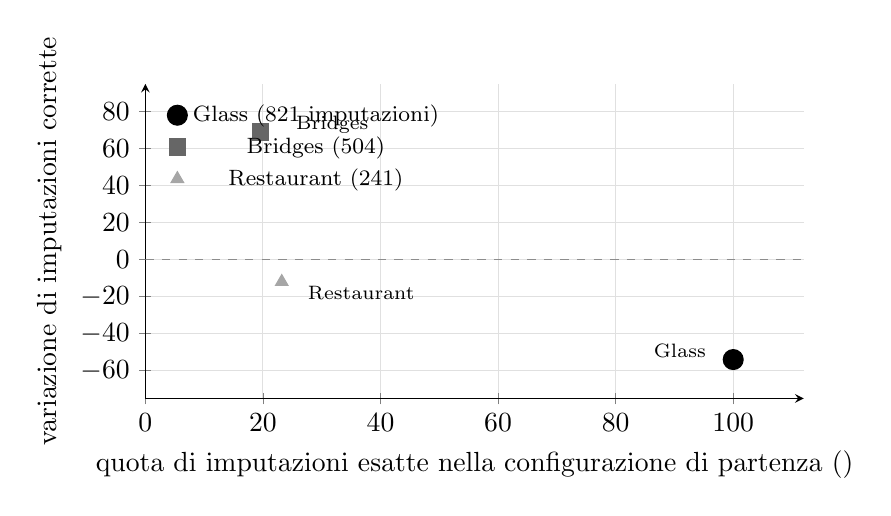
\begin{tikzpicture}
\begin{axis}[
    width=0.82\textwidth,
    height=0.46\textwidth,
    xlabel={quota di imputazioni esatte nella configurazione di partenza (\si{\percent})},
    ylabel={variazione di imputazioni corrette},
    xmin=0, xmax=112, ymin=-75, ymax=95,
    grid=major,
    grid style={black!12},
    axis lines=left,
    ytick={-60,-40,-20,0,20,40,60,80},
    xtick={0,20,40,60,80,100},
    legend style={font=\footnotesize, at={(0.02,0.97)}, anchor=north west, draw=none, fill=none},
]
\addplot[only marks, mark=*, mark size=3.6pt, color=black] coordinates {(100,-54)};
\addplot[only marks, mark=square*, mark size=3.0pt, color=black!60] coordinates {(19.6,69)};
\addplot[only marks, mark=triangle*, mark size=2.6pt, color=black!35] coordinates {(23.2,-12)};
\addlegendentry{Glass (821 imputazioni)}
\addlegendentry{Bridges (504)}
\addlegendentry{Restaurant (241)}
\draw[dashed, black!45] (axis cs:0,0) -- (axis cs:112,0);
\node[font=\scriptsize, anchor=west] at (axis cs:24,73) {Bridges};
\node[font=\scriptsize, anchor=west] at (axis cs:26,-18) {Restaurant};
\node[font=\scriptsize, anchor=east] at (axis cs:97,-49) {Glass};
\end{axis}
\end{tikzpicture}
\caption{Il meccanismo su tre famiglie. In ascissa la quota di imputazioni ottenute per via esatta
nella configurazione di partenza, in ordinata la variazione di imputazioni corrette prodotta dalla
potatura aggressiva; la dimensione del marcatore è proporzionale al numero di imputazioni della
configurazione di partenza. Il guadagno richiede che la quota esatta non sia satura: dove lo è
(Glass) la potatura può soltanto togliere copertura.}
\label{fig:mechanism}
\end{figure}

Le sezioni precedenti hanno stabilito \emph{che cosa} accade. Questa sezione stabilisce
\emph{perché}, e il risultato è il contributo interpretativo principale del lavoro.

Il sistema registra, per ogni imputazione effettuata, se essa sia stata ottenuta per via
\emph{esatta} --- la scorciatoia che si attiva quando la regola impiegata ha soglia di destra
nulla --- oppure per via approssimata. La distinzione era disponibile nei dati di tutte le
campagne, ma non era stata impiegata nell'interpretazione. La
\autoref{tab:mechanism} la mette in relazione con il numero di imputazioni.

\begin{table}[htbp]
\centering
\caption{Il meccanismo del guadagno. Per ciascuna famiglia si confrontano il numero di
imputazioni, la quota di quelle ottenute per via esatta e il numero di imputazioni corrette,
prima e dopo la potatura aggressiva. I valori sono aggregati sulla \emph{campagna completa} di
ciascuna famiglia: \num{50} configurazioni per Bridges, \num{45} per Glass, \num{18} per
Restaurant, alla taratura $\alpha = 0{,}85$.}
\label{tab:mechanism}
\footnotesize
\begin{tabular}{lrrrrr}
\toprule
& \multicolumn{2}{c}{\textbf{configurazione di partenza}} & \multicolumn{2}{c}{\textbf{dopo \str{A5b}}} & \\
\cmidrule(lr){2-3}\cmidrule(lr){4-5}
famiglia & imputazioni & quota esatta & imputazioni & quota esatta & $\Delta$ corrette \\
\midrule
Bridges (\num{50})    & \num{1309} & \SI{21.8}{\percent} & \num{1306} & \textbf{\SI{40.4}{\percent}} & $\mathbf{+69}$ \\
Glass (\num{45})      & 821        & \SI{100.0}{\percent} & 721       & \SI{100.0}{\percent}        & $-54$ \\
Restaurant (\num{18}) & 241        & \SI{23.2}{\percent}  & 229       & \textbf{\SI{49.8}{\percent}} & $-12$ \\
\bottomrule
\end{tabular}
\end{table}

Il numero di imputazioni corrette è il prodotto di due fattori: il \emph{numero} di imputazioni
effettuate e la \emph{quota} di quelle corrette, che a sua volta dipende dalla composizione dei
candidati e in particolare dalla quota di imputazioni ottenute per via esatta. La potatura
produce un guadagno soltanto se la composizione ha spazio per migliorare \emph{e} il numero di
imputazioni non diminuisce abbastanza da compensare il miglioramento. La
\autoref{tab:mechanism} mostra che i tre casi si distinguono esattamente su questo:

\begin{itemize}[leftmargin=1.4em]
    \item \textbf{Bridges}: la quota esatta cresce dal \SI{21.8}{\percent} al \SI{40.4}{\percent}
    e il numero di imputazioni resta sostanzialmente invariato (\num{1309} contro \num{1306}). Il
    miglioramento della composizione si trasferisce integralmente al risultato: \num{69}
    imputazioni corrette in più.
    \item \textbf{Glass}: la quota esatta è \emph{già} pari al \SI{100}{\percent}, perché ogni
    imputazione passa per la via esatta. Non vi è spazio per migliorare la composizione, e la
    potatura può soltanto togliere copertura: le imputazioni scendono da \num{821} a \num{721} e
    le corrette da \num{517} a \num{463}.
    \item \textbf{Restaurant}: la composizione ha spazio e migliora più che su Bridges (dal
    \SI{23.2}{\percent} al \SI{49.8}{\percent}), ma il numero di imputazioni cala da \num{241} a
    \num{229} e le imputazioni guadagnate in composizione sono meno di quelle perse in copertura:
    il saldo è di \num{12} imputazioni corrette in meno.
\end{itemize}

Sulle \num{20} configurazioni comuni all'ablazione, dove entrambi i bracci sono misurati sulle
stesse configurazioni, i due fattori crescono entrambi e la variazione è di $+45$
(\autoref{tab:ablation}): la differenza rispetto al $+69$ della campagna completa è una
differenza di campione, non di strategia, ed è la ragione per cui le due tabelle dichiarano
ciascuna la propria base.

Questo risultato spiega anche un'osservazione che era rimasta senza interpretazione: il riordino
\str{exact-priority} è risultato un \emph{no-op esatto} su Glass, con output identico in
\num{45} configurazioni su \num{45}. La spiegazione è immediata una volta nota la quota esatta:
se tutte le imputazioni passano già per la via esatta, non vi è alcuna regola da promuovere.

\paragraph{Perché la sinergia non è misteriosa.} La \autoref{tab:ablation} --- che si riferisce
alle \num{20} configurazioni comuni ai quattro bracci --- mostra che il guadagno della
combinazione ($+45$) supera di molto la somma dei componenti isolati ($+5$). Il meccanismo rende
conto della differenza: i due componenti agiscono su fattori \emph{diversi}. Il riordino per
priorità di precisione dispone per prime le regole che producono valori esatti, e migliora quindi
la composizione dei candidati; la potatura adattiva modifica quali regole concorrono alla
generazione, e quindi quante celle trovano un candidato accettabile. Ciascun componente vale
tanto più quanto più è alto il fattore su cui l'altro agisce, e la combinazione è per questo
super-additiva: è la stessa legge dei due fattori, letta sul campione in cui entrambi sono
misurati.

% =======================================================================================
\section{Il criterio diagnostico}\label{sec:diagnostic}

\begin{figure}[htbp]
\centering
\begin{tikzpicture}[
    font=\footnotesize,
    node distance=7mm,
    st/.style={draw, rounded corners=1pt, align=center, inner sep=4pt, minimum height=8mm},
    dec/.style={draw, diamond, aspect=2.6, align=center, inner sep=1pt, font=\scriptsize},
    ar/.style={-{Latex[length=2mm]}, thick}
]
\node[st] (m1) {misura la quota esatta\\della configurazione di partenza};
\node[dec, below=of m1] (d1) {quota $\approx \SI{100}{\percent}$?};
\node[st, right=14mm of d1] (no1) {\textbf{non potare}\\la leva non esiste};
\node[st, below=of d1] (m2) {applica la strategia e misura\\la copertura su un sottoinsieme};
\node[dec, below=of m2] (d2) {la copertura cala?};
\node[st, right=14mm of d2] (no2) {taratura conservativa\\o nessuna potatura};
\node[st, below=of d2, fill=black!10] (ok) {\textbf{adotta la potatura}};
\draw[ar] (m1) -- (d1);
\draw[ar] (d1) -- node[above, font=\scriptsize] {sì} (no1);
\draw[ar] (d1) -- node[right, font=\scriptsize] {no} (m2);
\draw[ar] (m2) -- (d2);
\draw[ar] (d2) -- node[above, font=\scriptsize] {sì} (no2);
\draw[ar] (d2) -- node[right, font=\scriptsize] {no} (ok);
\end{tikzpicture}
\caption{Procedura del criterio diagnostico. Il primo passo non richiede esecuzioni, perché la
quota esatta è registrata dal sistema; il secondo richiede di misurare la copertura, ed è il solo
costo del criterio.}
\label{fig:criterion}
\end{figure}

Dal meccanismo discende un criterio operativo, che sostituisce la soglia euristica adottata in
precedenza. Il criterio si fonda su una grandezza che il sistema \emph{registra già}: la quota di
imputazioni ottenute per via esatta nella configurazione di partenza, disponibile nei file di
risultato prima di qualunque potatura.

\begin{description}[leftmargin=0em]
    \item[Quota esatta $\approx \SI{100}{\percent}$.] La leva della qualità non esiste: non vi è
    margine per sostituire imputazioni approssimate con imputazioni esatte, e la potatura può
    soltanto togliere copertura. \emph{Non potare}. È il caso di Glass.
    \item[Quota esatta bassa.] La leva esiste, e la potatura conviene \emph{a condizione che la
    copertura non cali}. È il caso di Bridges, dove la copertura cresce, e di Restaurant, dove
    cala.
\end{description}

\paragraph{La procedura.} Il criterio si traduce in quattro passi, eseguibili senza modificare né
il sistema né il dataset.

\begin{enumerate}[leftmargin=1.6em]
    \item \textbf{Misurare la quota esatta} della configurazione di partenza, leggendola dai file
    di risultato che il sistema produce comunque: il costo di questo passo è nullo, perché non
    richiede esecuzioni aggiuntive.
    \item \textbf{Decidere se la leva esiste.} Una quota prossima al \SI{100}{\percent} la
    esclude, e la decisione è di non potare; una quota bassa lascia la leva aperta, e si prosegue.
    \item \textbf{Misurare la copertura su un sottoinsieme} di configurazioni, applicando la
    strategia e confrontando il numero di celle valorizzate con quello della configurazione di
    partenza. È il solo passo che richieda esecuzioni, ed è quindi il costo del criterio.
    \item \textbf{Adottare la potatura solo se la copertura non cala}; in caso contrario ricorrere
    alla taratura conservativa, che riduce il rischio rinunciando a parte della riduzione.
\end{enumerate}

\paragraph{Che cosa il criterio decide e che cosa no.} Il primo termine --- se la leva esista --- è
decidibile a costo nullo e prima di qualunque esecuzione. Il secondo --- se la copertura calerà
--- non è prevedibile senza eseguire il sistema, e il criterio non è quindi sufficiente a decidere
in autonomia: la sua funzione è di \emph{escludere} i casi in cui la potatura non può che
danneggiare, non di autorizzarla. La \autoref{tab:criterion} riassume le tre famiglie su cui il
criterio è stato derivato.

\begin{table}[htbp]
\centering
\caption{Applicazione del criterio alle tre famiglie su cui è stato derivato. Le grandezze a
cui il criterio si riferisce sono quelle della \autoref{tab:mechanism}, che non vengono qui
ripetute. La tabella documenta i casi da cui il criterio è stato ricavato e non costituisce una
sua validazione: la prova su una famiglia indipendente è riportata nella
\autoref{sec:physician}.}
\label{tab:criterion}
\footnotesize
\begin{tabular}{@{}lp{4.5cm}p{5.4cm}@{}}
\toprule
famiglia & decisione del criterio & esito osservato \\
\midrule
Glass & \emph{non potare}: la leva non esiste & coerente: la potatura toglie copertura senza poter migliorare la composizione \\
Bridges & \emph{potare se la copertura tiene} & coerente: la copertura resta invariata e il risultato migliora \\
Restaurant & \emph{misurare prima di adottare} & coerente: la copertura cala e il risultato peggiora \\
\bottomrule
\end{tabular}
\end{table}

\paragraph{Perché il criterio non è una soglia adattata ai dati.} La grandezza impiegata non è un
punteggio scelto per separare i casi favorevoli da quelli sfavorevoli, ma il termine che il
meccanismo indica come necessario: il guadagno è il prodotto della quota esatta e del numero di
imputazioni, e una quota esatta pari al \SI{100}{\percent} annulla il primo fattore per
definizione. La soglia al \SI{100}{\percent} non è quindi un parametro da tarare; la zona
intermedia --- quote basse ma non nulle --- resta però indeterminata, ed è il limite principale
del criterio.

% =======================================================================================
\section{La prova sulla quarta famiglia}\label{sec:physician}

Il criterio della sezione precedente è stato derivato su tre famiglie. Il test che servirebbe è su
una famiglia mai impiegata, e l'archivio ne contiene una: la famiglia Physician, il cui schema è
allineato ai propri file di regole. La prova è stata condotta su tutto il materiale eseguibile, e
il suo esito è \emph{parzialmente conclusivo}: conferma l'equivalenza della potatura garantita e
fornisce due casi coerenti con il criterio, ma su un numero di celle troppo piccolo per fondare
una conclusione statistica.

\paragraph{Perché le configurazioni piene non sono impiegabili.} I dataset non remodulati
contengono \num{103592} righe e fino a \num{121913} celle nulle. La ragione dell'impraticabilità
non è però il tempo di imputazione: è il \emph{preprocessing interno} del sistema, che all'avvio
verifica per ciascuna regola a soglia di destra nulla se il suo lato sinistro si comporti da
chiave, con un confronto a coppie di tuple quadratico nel numero di righe
(\autoref{sec:dual-role}). La sonda condotta sulla configurazione più piccola
(\texttt{Physician\_Compare\_National\_13467\_1}, \num{13467} celle) è stata interrotta dopo
\SI{1200}{\second} senza che il sistema avesse prodotto \emph{una sola} riga di risultato: il
tempo era ancora interamente assorbito dal preprocessing. La circostanza è coerente con il
materiale d'archivio, che per la medesima configurazione contiene un file di risultati parziale di
\num{1005} righe e un file di celle popolate vuoto.

\paragraph{Che cosa è stato possibile eseguire.} Delle quattro versioni remodulate, due --- 0.05 e
0.1 --- non sono eseguibili per il difetto D3 (\autoref{sec:d3}): il sistema si arresta
all'avvio su righe del dataset con un numero di campi inferiore allo schema. Le due versioni
eseguibili, 0.005 e 0.01, valutano \num{13} e \num{27} celle; escludendo dalle altre due le celle
non localizzabili, il materiale eseguibile salirebbe a \num{329} celle, ma la riparazione delle
righe malformate non è stata applicata perché il costo di preprocessing la rende non conveniente
rispetto al contributo ottenibile (\autoref{sec:d3}).

\paragraph{Verifica di equivalenza.} La potatura garantita è stata applicata a tutte le
configurazioni eseguibili, con la politica di tutela integrale dei veti. L'esito è netto: su
\num{2} configurazioni su \num{2} i file delle celle popolate e dei risultati sono
\emph{byte-identici} a quelli della configurazione di partenza, con riduzioni dell'insieme di
regole del \SI{6}{\percent} e del \SI{5}{\percent}. È la prima verifica della condizione \Vtwo{}
su una famiglia indipendente da quelle su cui è stata derivata, e si aggiunge alle \num{111}
configurazioni già verificate.

\paragraph{Il test del criterio.} La \autoref{tab:res-physician} riporta i due casi eseguibili.

\begin{table}[htbp]
\centering
\caption{Prova esplorativa sulla famiglia Physician. Confronto fra configurazione di partenza e
potatura aggressiva sulle due versioni eseguibili; ``esatte'' sono le imputazioni ottenute per via
esatta, ``corrette'' quelle conformi al ground truth.}
\label{tab:res-physician}
\footnotesize
\begin{tabular}{lrrrrrrr}
\toprule
versione & celle & imputate & esatte & quota esatta & corrette & copertura & riduzione \\
\midrule
0.005, partenza & 13 & 3 & 3 & \SI{100}{\percent} & 2 & \SI{23.1}{\percent} & --- \\
0.005, \str{A5b} & 13 & 3 & 3 & \SI{100}{\percent} & 2 & \SI{23.1}{\percent} & \SI{67}{\percent} \\
0.01, partenza  & 27 & 11 & 5 & \SI{45}{\percent} & 4 & \SI{40.7}{\percent} & --- \\
0.01, \str{A5b}  & 27 & 9 & 3 & \SI{33}{\percent} & 3 & \SI{33.3}{\percent} & \SI{74}{\percent} \\
\bottomrule
\end{tabular}
\end{table}

I due casi hanno esiti diversi e istruttivi. Sulla versione 0.005 la configurazione di partenza
ottiene \emph{tutte} le proprie imputazioni per via esatta: la leva della qualità non esiste, il
criterio prescrive di non potare, e la potatura aggressiva --- pur rimuovendo due terzi delle
regole --- non cambia nulla. Sulla versione 0.01 la quota esatta di partenza è del
\SI{45}{\percent}, la leva esiste, e la potatura \emph{peggiora} il risultato: le celle valorizzate
scendono da \num{11} a \num{9}, le imputazioni esatte da \num{5} a \num{3}, le corrette da \num{4}
a \num{3}. Il criterio prescrive in questo caso di misurare la copertura prima di adottare la
potatura, e la misura dice di non adottarla.

Entrambi gli esiti sono quindi coerenti con il criterio, uno per esclusione della leva e uno per
caduta della copertura. Il valore probatorio resta però limitato, per tre ragioni che vanno
dichiarate: le celle valutabili sono \num{40} in tutto; la soglia disponibile è una sola
(\num{3}, l'unica per cui l'archivio contenga i file di regole); e su questa famiglia il sistema
imputa una frazione minoritaria delle celle, cosicché le differenze osservate valgono poche unità.
La prova va letta come un \emph{controllo di coerenza} su dati nuovi, non come una validazione.

\section{Risultati negativi}\label{sec:negative-results}

Una parte rilevante delle strategie sperimentate non ha prodotto il guadagno atteso. I risultati
sono riportati perché delimitano lo spazio delle soluzioni.

\paragraph{Il segnale di precisione non è la causa del guadagno del riordino.}
Il riordino dei cluster per precisione empirica produce un guadagno misurabile
($+96$ imputazioni corrette su \num{30} configurazioni, $p = 2.5\cdot 10^{-6}$). L'ipotesi che tale
guadagno fosse attribuibile al segnale di precisione è stata sottoposta a un esperimento di
controllo: a parità di insieme di regole, si sono confrontati l'ordinamento per precisione,
l'ordinamento inverso e tre permutazioni casuali indipendenti.

\begin{table}[htbp]
\centering
\caption{Esperimento di controllo sull'ordinamento dei cluster. Quindici configurazioni, cinque
bracci, insieme di regole invariato.}
\label{tab:res-order}
\footnotesize
\begin{tabular}{lrrrr}
\toprule
braccio & corrette & $\Delta$ vs orig.\ & migl.\ / pegg.\ & Wilcoxon \\
\midrule
originale                      & 333 & ---    & --- & --- \\
riordino per precisione        & 386 & $+53$  & 13 / 0 & $p = \num{0.0016}$ \\
permutazione casuale (media di 3) & --- & $+52.7$ & 13 / 0 & $p = \num{0.0016}$ \\
riordino inverso               & 313 & $-20$  & 6 / 1 & $p = \num{0.2702}$ \\
\bottomrule
\end{tabular}
\end{table}

Il confronto decisivo è fra il riordino per precisione e la permutazione casuale: la differenza è
$+0.33$ imputazioni corrette, con $p = \num{0.8878}$, e una delle permutazioni casuali supera
l'ordinamento per precisione. Il guadagno \emph{non è attribuibile al segnale impiegato}. Il
riordino inverso, d'altra parte, peggiora il risultato rispetto all'originale: non è dunque vero
che qualunque permutazione funzioni, ma che l'ordine di partenza è prossimo al caso peggiore e
che qualunque ordine che non sia l'inverso lo migliora.

\paragraph{La regolarizzazione della stima non ha effetto.} La sostituzione della stima di
precisione con una stima contratta verso un valore a priori è stata sperimentata su quattro
valori del parametro di contrazione. I risultati sono \emph{identici} in tutte le
configurazioni per tutti i valori: il parametro non è una variabile da tarare.

\paragraph{Il riordino entro il cluster è inerte per costruzione.} La procedura che genera i
candidati percorre tutte le regole di un cluster e ne conserva il minimo, senza uscite
anticipate. L'ordine interno al cluster non può quindi influenzare il valore imputato. La
previsione è stata confermata empiricamente su \num{15} configurazioni su \num{15}, con zero
differenze non nulle al test.

\paragraph{L'ordinamento delle rimozioni sotto vincolo di budget è un vicolo cieco.} La politica
\str{budget:F} ordina le regole da rimuovere secondo un indice di rischio. Tale indice è risultato
\emph{anti-correlato} con la rilevanza effettiva delle regole: su \num{8961} regole, la
correlazione di rango con il numero di celle che ciascuna regola può servire è $\rho = -0.237$.
La causa è stata individuata: l'indice somma i valori mancanti sulle colonne del lato
\emph{sinistro}, mentre una regola può servire soltanto celle della propria colonna di
\emph{destra}. La correzione dell'indice produce un miglioramento strutturale netto --- a parità
di budget, rimuove $2.5$ volte più regole che non servono alcuna cella e distrugge $2.6$ volte
meno celle servibili --- ma il vantaggio \emph{non si traduce in un miglioramento dell'esito}:
su \num{13} configurazioni distribuite su tre famiglie, il saldo delle imputazioni corrette è
identico. La conclusione è che, sotto vincolo di budget, conta la \emph{dimensione} del budget e
non l'\emph{ordine} con cui si sceglie.

\paragraph{Una potatura esatta della generazione può rallentare il sistema.} La strategia
\str{score-argmin}, che preserva la generazione calcolando staticamente quali regole non sono mai
l'argomento del minimo, raggiunge riduzioni fino al \SI{98}{\percent} e preserva la copertura.
Rende però l'esecuzione fino a \num{251} volte più lenta. Il risultato mostra che la relazione fra
numero di regole e tempo di esecuzione non è monotona, e che la riduzione non è di per sé un
indicatore di efficienza.

% =======================================================================================
\section{Il costo: perché ridurre non basta}\label{sec:res-cost}\label{sec:score-argmin}

\begin{figure}[htbp]
\centering
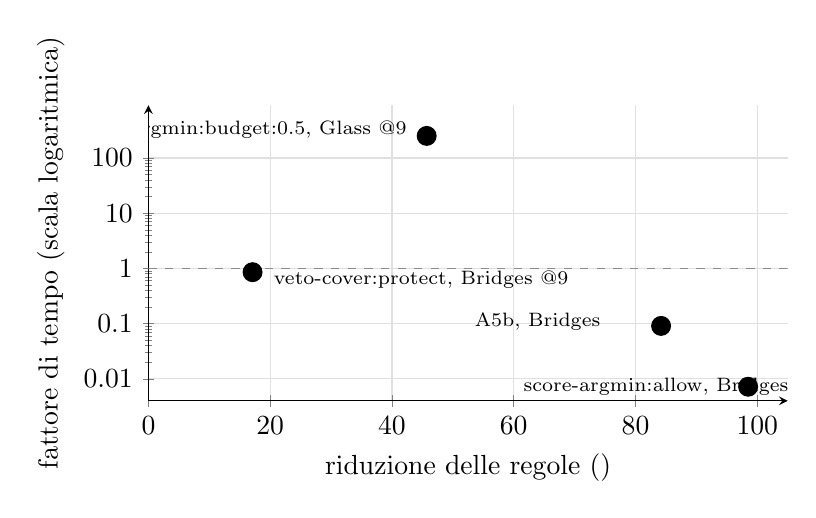
\begin{tikzpicture}
\begin{axis}[
    width=0.80\textwidth,
    height=0.44\textwidth,
    xlabel={riduzione delle regole (\si{\percent})},
    ylabel={fattore di tempo (scala logaritmica)},
    xmin=0, xmax=105,
    ymode=log,
    ymin=0.004, ymax=900,
    ytick={0.01,0.1,1,10,100},
    yticklabels={$0.01$, $0.1$, $1$, $10$, $100$},
    grid=major,
    grid style={black!12},
    axis lines=left,
]
\addplot[only marks, mark=*, mark size=3.4pt, color=black]
    coordinates {(98.5,0.0072) (84.2,0.091) (17.1,0.855) (45.7,251)};
\draw[dashed, black!45] (axis cs:0,1) -- (axis cs:105,1);
\node[font=\scriptsize, anchor=west] at (axis cs:60,0.0072) {\str{score-argmin:allow}, Bridges @15};
\node[font=\scriptsize, anchor=west] at (axis cs:52,0.11) {\str{A5b}, Bridges};
\node[font=\scriptsize, anchor=west] at (axis cs:19,0.62) {\str{veto-cover:protect}, Bridges @9};
\node[font=\scriptsize, anchor=east] at (axis cs:44,330) {\str{score-argmin:budget:0.5}, Glass @9};
\end{axis}
\end{tikzpicture}
\caption{Riduzione ottenuta e fattore di tempo per quattro casi misurati. Il fattore è il rapporto
fra il tempo di esecuzione della configurazione potata e quello della configurazione di partenza:
valori inferiori a uno indicano un'accelerazione. La relazione fra le due grandezze non è
monotona, e il caso con la riduzione maggiore è anche il più veloce mentre un caso con riduzione
inferiore è il più lento.}
\label{fig:time}
\end{figure}

L'ipotesi H16 prevedeva che il tempo di esecuzione seguisse il numero di regole rimosse. I dati la
falsificano, e il modo in cui la falsificano è più interessante della previsione.

Il costo di \emph{preprocessing} della potatura non è invece in discussione: la riscrittura del
file delle regole è trascurabile rispetto all'esecuzione del sistema e cresce con il numero di
regole, attestandosi nell'ordine dei secondi sui file maggiori (\num{27445} regole). Il confronto
fra i due costi è quindi interamente a favore della potatura, e il problema non è il costo
dell'analisi ma l'effetto sull'esecuzione.

\str{score-argmin} rimuove fino al \SI{98}{\percent} delle regole e rende il sistema
\emph{drammaticamente più lento}: il rallentamento mediano è di \num{5.8} volte con la variante
\str{allow} e di \num{20.1} volte con \str{budget:0.5}, con un massimo di \num{251} volte sulla
configurazione \texttt{glass\_43\_2} a soglia 9, dove il tempo di esecuzione passa da
\SI{3.5}{\second} a \SI{873}{\second} mentre le regole scendono da \num{11648} a \num{6323}. Su
quattordici configurazioni, la variante \str{allow} è più veloce della configurazione di partenza
in \emph{una sola}.

\begin{table}[htbp]
\centering
\caption{Rallentamento del tempo di esecuzione prodotto da \str{score-argmin} su Glass, rispetto
alla configurazione di partenza. Il rallentamento è il rapporto fra il tempo della variante potata
e quello della variante non potata, sulla stessa configurazione.}
\label{tab:res-slowdown}
\footnotesize
\begin{tabular}{lrr}
\toprule
variante & rallentamento mediano & rallentamento massimo \\
\midrule
\str{score-argmin:allow}       & \num{5.8}$\times$  & \num{28}$\times$ \\
\str{score-argmin:budget:0.5}  & \num{20.1}$\times$ & \num{251}$\times$ \\
\bottomrule
\end{tabular}
\end{table}

La circostanza che esclude la spiegazione ovvia è un confronto interno alla tabella: la variante
\str{budget:0.5} \emph{conserva più regole} di \str{allow} --- \num{6323} contro \num{1098} sulla
configurazione citata --- ed è circa nove volte più lenta. Non è dunque la \emph{quantità} delle
regole a determinare il tempo, ma la loro \emph{composizione}: il tempo dipende da quali regole
sopravvivono, non da quante.

Una spiegazione candidata esiste ed è coerente con l'analisi del sistema, ma \emph{non è
verificata} e va presentata come tale. Il sistema dispone di una scorciatoia esatta che chiude una
cella in tempo costante quando la tupla presenta una sola cella nulla e la regola impiegata ha
soglia di destra nulla (\autoref{sec:two-branches}). Se l'insieme potato non contiene più le regole
che attivano quella scorciatoia per la maggior parte delle celle, ogni cella ricade nella ricerca
per similarità sull'intero dataset, il cui costo è lineare nel numero di righe anziché costante.
La potatura rimuoverebbe cioè, insieme alle regole dannose, la via rapida. La verifica richiede di
strumentare il percorso della scorciatoia, che non è stato possibile isolare con la
strumentazione disponibile, e la questione è registrata fra gli sviluppi
(\autoref{sec:future-work}).

La conseguenza pratica è netta ed è il motivo per cui la sezione è necessaria: \str{score-argmin}
non è una strategia utilizzabile, malgrado il criterio esatto che la fonda e la conferma
sperimentale della sua proprietà principale. Un guadagno di copertura pagato con un tempo di
esecuzione da sei a duecentocinquanta volte maggiore non è un compromesso proponibile. Il caso
mostra inoltre che la domanda del lavoro --- se la potatura migliori \emph{e} acceleri --- non
ammette una risposta unica: le due grandezze possono muoversi in direzioni opposte, e la
valutazione di una strategia deve riportarle entrambe.

% =======================================================================================
